% =====================================================================
% AI Academy -- National AI Center
% Software Engineering Final Project -- Team Report Template
%
% HOW TO USE
% ----------
%   1. Edit the CONFIGURATION block below (team name, topic, members).
%   2. Replace every [TODO: ...] with your content. TODOs render in red,
%      so anything you forgot will be visually obvious in the PDF.
%   3. Three kinds of cues throughout:
%        - REQUIRED DELIVERABLE box (blue): exactly what we expect.
%        - PROBING QUESTIONS box (amber): NOT a checklist; these are
%          prompts that should shape how you write the section. A strong
%          response engages with at least 2 of them; a weak response
%          ignores them all.
%        - "Your response:" placeholders: replace with your text/diagram.
%   4. Target length: 8-10 pages including figures, excluding bibliography.
%   5. Compile with pdfLaTeX. Overleaf works out of the box.
% =====================================================================

\documentclass[11pt,a4paper]{article}

% ===== EARLY MACROS (must come before configuration) =================
% (Full styling lower down; we just need \TODO and \ph available
% before the configuration block uses them.)
\usepackage[dvipsnames]{xcolor}
\definecolor{accent2}{HTML}{8B0000}
\definecolor{ph}{HTML}{6B7280}
\newcommand{\TODO}[1]{\textcolor{accent2}{\textbf{[TODO: #1]}}}
\newcommand{\phh}[1]{\textcolor{ph}{\textit{#1}}}

% ===== CONFIGURATION (edit these) ====================================
\newcommand{\teamname}{AI Food Analyzer Team}
\newcommand{\topicchoice}{Topic 2 -- AI Food Analyzer}
\newcommand{\member}[2]{\textbf{#1} (#2)}  % name, GitHub handle
\newcommand{\reportdate}{19 September 2026}
\newcommand{\repolink}{\url{https://github.com/budagovfn/ai-food-analyzer}}

% ===== course meta (rarely changes) ==================================
\newcommand{\coursecode}{AI-ENG-110}
\newcommand{\coursename}{Software Engineering}
\newcommand{\institution}{AI Academy, National AI Center}
\newcommand{\semester}{Spring 2026}

% ===== PACKAGES ======================================================
\usepackage[margin=2.2cm,headheight=15pt]{geometry}
\usepackage[T1]{fontenc}
\usepackage[utf8]{inputenc}
\usepackage[final,protrusion=true,expansion=false]{microtype}
\usepackage{amsmath,amssymb}
\usepackage{graphicx}
\usepackage{booktabs}
\usepackage{array}
\usepackage{tabularx}
\usepackage{ragged2e}
\usepackage{enumitem}
\usepackage[parfill]{parskip}
\usepackage{listings}
\usepackage[most]{tcolorbox}
\usepackage{titlesec}
\usepackage{fancyhdr}
\usepackage{lastpage}
\usepackage{tikz}
\usetikzlibrary{shapes.geometric,arrows.meta,positioning,fit,backgrounds,calc}
\usepackage[hidelinks]{hyperref}

\emergencystretch=3em
\hbadness=10000
\hfuzz=2pt

\hypersetup{
  colorlinks=true,
  linkcolor=NavyBlue,
  urlcolor=NavyBlue,
  citecolor=NavyBlue,
  pdftitle={\coursecode\ Final Project Report},
  pdfauthor={\teamname}
}

% ===== STYLING =======================================================
\definecolor{accent}{HTML}{0B3D91}
\definecolor{soft}{HTML}{F2F4F8}
\definecolor{deliver}{HTML}{E8F0FE}
\definecolor{deliverframe}{HTML}{1A56DB}
\definecolor{probe}{HTML}{FFF8E1}
\definecolor{probeframe}{HTML}{B45309}

\titleformat{\section}
  {\Large\bfseries\color{accent}}{\thesection.}{0.6em}{}
\titleformat{\subsection}
  {\large\bfseries\color{accent}}{\thesubsection}{0.5em}{}

\newcommand{\ans}[1]{\rule[-2pt]{#1}{0.5pt}}
\let\ph\phh  % alias the early \phh as \ph for consistency with the body

% Deliverable callout (light blue)
\newtcolorbox{deliverbox}{
  colback=deliver, colframe=deliverframe, boxrule=0.5pt,
  arc=2pt, left=8pt, right=8pt, top=4pt, bottom=4pt
}
% Probing-question callout (light amber)
\newtcolorbox{probebox}{
  colback=probe, colframe=probeframe, boxrule=0.5pt,
  arc=2pt, left=8pt, right=8pt, top=4pt, bottom=4pt
}

\definecolor{codegreen}{rgb}{0,0.55,0}
\definecolor{codegray}{rgb}{0.4,0.4,0.4}
\definecolor{codepurple}{rgb}{0.55,0,0.78}
\definecolor{backcolour}{rgb}{0.97,0.97,0.97}

\lstdefinestyle{python}{
  language=Python,
  backgroundcolor=\color{backcolour},
  commentstyle=\color{codegreen},
  keywordstyle=\color{accent},
  numberstyle=\tiny\color{codegray},
  stringstyle=\color{codepurple},
  basicstyle=\ttfamily\footnotesize,
  breakatwhitespace=false,
  breaklines=true,
  keepspaces=true,
  numbers=left,
  numbersep=6pt,
  tabsize=2,
  frame=single,
  framerule=0.4pt,
  rulecolor=\color{black!30},
}

\pagestyle{fancy}
\fancyhf{}
\fancyhead[L]{\small\textit{\coursecode\ -- Final Report -- \teamname}}
\fancyhead[R]{\small\textit{\semester}}
\fancyfoot[L]{\small\textit{\institution}}
\fancyfoot[R]{\small Page \thepage\ of \pageref{LastPage}}
\renewcommand{\headrulewidth}{0.4pt}
\renewcommand{\footrulewidth}{0.4pt}

% =====================================================================
\begin{document}

\begin{center}
{\small \textsc{\institution} \\[0.2em] \textsc{\coursecode\ -- \coursename\ -- \semester}}\\[1.2em]
{\Large\bfseries\color{accent} Final Project Report}\\[0.3em]
{\LARGE\bfseries \topicchoice}\\[0.6em]
\rule{0.85\textwidth}{0.6pt}
\end{center}

\vspace{0.6em}
\begin{tabularx}{\textwidth}{@{}lXlX@{}}
\textbf{Team:} & \teamname & \textbf{Date:} & \reportdate \\
\textbf{Repo:} & \repolink & \textbf{Tag:} & \texttt{v1.0-final} \\
\textbf{Members:} & \multicolumn{3}{X@{}}{%
  \member{Farhad Budagov}{@budagovfn},\quad
  \member{Mikayil Hasanov}{@mickael044},\quad
  \member{Nihad Gojayev}{@justpr09rammer}
}\\
\end{tabularx}
\vspace{0.4em}\hrule\vspace{0.6em}

% ===== EXECUTIVE SUMMARY =============================================
\section*{Executive Summary}
\addcontentsline{toc}{section}{Executive Summary}

We built the software-engineering layer around the course-provided AI module for Topic 2: a system that takes a photo of a meal, identifies its ingredients and estimated portion sizes through a vision-language model, looks up the nutrition facts for every ingredient in parallel, and returns total calories and a macronutrient breakdown through both a command-line tool and an HTTP API, with every analysis persisted to PostgreSQL. Nutrition lookups for the ingredients in one photo run concurrently through \texttt{asyncio.gather} bounded by a semaphore of 10, instead of one HTTP call at a time; on our measured 10-ingredient workload this took the pipeline from 15.69s sequentially to 3.16s concurrently, a \textbf{4.96$\times$} speedup (\S\ref{sec:concurrency}). Our clearest robustness story came from a real bug, not a synthetic one: on Windows, writing the uploaded photo to an auto-deleted temporary file and then handing its path back to the AI module (which reopens the file by path) crashed every single \texttt{POST /analyze} request with a native \texttt{PermissionError}, because Windows will not let a second handle open a file that is still held open by the first -- we root-caused it from the traceback, switched to a permanent, explicitly-cleaned-up upload path, and it has not recurred since (\S\ref{sec:robustness}). The most surprising thing the team learned was how much of "robustness" in practice is about the boring, unglamorous failure modes -- a stale API key returning a silent \texttt{403}, a provider having a transient outage unrelated to our own code, a Windows-only file-locking quirk -- rather than the exotic ones we originally worried about (malformed JSON from the model, adversarial inputs). If we started over, we would write the HTTP and CLI entry-point tests before, not after, the API itself, since that is exactly the gap that kept our coverage below the 60\% target.

% ===== TABLE OF CONTENTS =============================================
\tableofcontents
\vspace{0.6em}\hrule\vspace{0.4em}

% =====================================================================
\section{Project Overview}

\subsection{Problem framing \& scope}

A user has a photo of a meal and wants to know, without weighing anything or looking anything up by hand, roughly how many calories and how much protein, carbohydrate and fat it contains. Our system takes that photo as input and returns a structured breakdown: a list of the ingredients the model recognized, each with an estimated weight in grams and a confidence score, and the total kcal/protein/carbs/fat for the whole meal. Every analysis is also written to a persistent history table so the user (or, later, an analytics feature) can look back over past meals.

There are two user-facing entry points. The CLI, run as \texttt{python -m foodanalyzer analyze <path> [--no-save]} and \texttt{python -m foodanalyzer history [--limit N]}, is meant for local, one-off use and prints an aligned text table. The HTTP API, run with \texttt{uvicorn src.api:app}, exposes \texttt{POST /analyze} (multipart image upload, JSON response) and \texttt{GET /health}, and is meant to be the front door for anything other than a terminal -- a future web or mobile client, for instance. Both entry points share exactly the same business logic underneath (identify $\rightarrow$ look up nutrition $\rightarrow$ compute totals $\rightarrow$ persist); the only thing that differs is how the image arrives and how the result is rendered.

Our provider stack is Gemini (\texttt{gemini-3.6-flash}) for ingredient identification and USDA FoodData Central for nutrition lookups, both reached exclusively through the provided \texttt{ai} package -- we never call \texttt{google-genai} or the USDA REST API directly. We did not use an embedding provider or a web-search provider; Topic 2 does not call for either. Where we tightened the spec: TOPIC.md's recommended layout suggests \texttt{src/services/ai\_service.py}, \texttt{src/concurrency/pipeline.py} and a separate \texttt{src/core/analyzer.py} for business logic; we flattened this to \texttt{src/ai\_service.py} and \texttt{src/pipeline.py} directly under \texttt{src/}, and folded the "core" orchestration straight into \texttt{cli.py}/\texttt{api.py} rather than adding an extra indirection layer, because with only two real business-logic steps (identify, then look up nutrition) a separate analyzer module added a file without adding clarity. Where we loosened it: the spec asks for a full token-bucket or leaky-bucket rate limiter; we shipped a bounded semaphore (\texttt{asyncio.Semaphore(10)}) plus retry-with-backoff instead, and say so plainly in \S\ref{sec:concurrency} rather than claiming a rate limiter we did not build.

\subsection{Provider choice and the AI module contract}

We used Google Gemini (\texttt{LLM\_PROVIDER=gemini}, \texttt{LLM\_MODEL=gemini-3.6-flash}) as the vision-language model and USDA FoodData Central (\texttt{NUTRITION\_PROVIDER=usda}) as the nutrition source; we used no embedding provider. From our own code we call exactly three functions from the provided package: \texttt{ai.identify\_ingredients} (wrapped by \texttt{src/ai\_service.py}), \texttt{ai.get\_nutrition\_provider()\allowbreak.lookup} (wrapped by the same module's \texttt{NutritionService}), and \texttt{ai.compute\_totals} (called directly from \texttt{src/cli.py} and \texttt{src/api.py} once nutrition facts are available). We confirm that the public interface of \texttt{ai/} was never modified -- every fix and every piece of validation lives in \texttt{src/}.

Response validation is mostly inherited for free: \texttt{ai.identify\_ingredients} already returns typed \texttt{Ingredient} / \texttt{NutritionFacts} pydantic objects rather than raw JSON, so a malformed or semantically-wrong payload (a negative weight, a missing field) fails pydantic validation \emph{inside} the provided module and surfaces to us as a \texttt{ProviderError}, which our retry policy (\S\ref{sec:robustness}) treats the same as any other transient provider failure. The one semantically-valid-but-empty case we do handle explicitly is "no meal recognized": \texttt{identify\_ingredients} returns \texttt{[]} rather than raising, and both entry points treat that as a normal control-flow branch (\texttt{AnalysisResponse(meal\_recognized=False, ...)} on the API, a plain printed message on the CLI) instead of an error.

% =====================================================================
\section{Architecture}\label{sec:arch}

\subsection{Module map}

\begin{center}
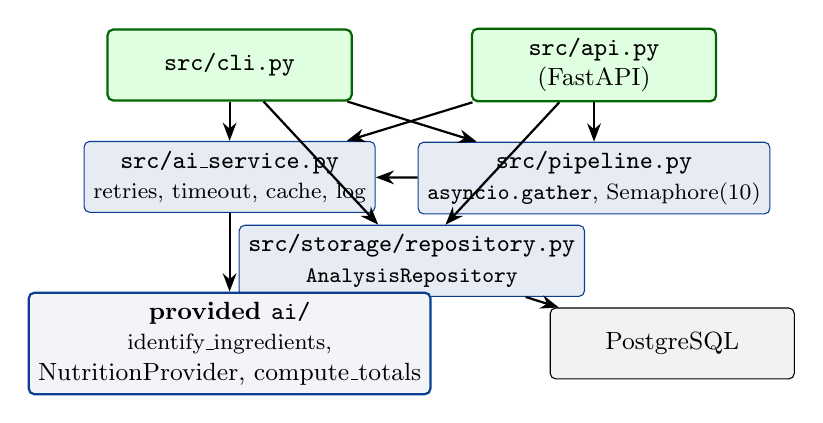
\begin{tikzpicture}[
  node distance=5mm,
  box/.style={draw,rounded corners=2pt,minimum width=3.1cm,minimum height=0.9cm,align=center,font=\small},
  aibox/.style={box,fill=soft,draw=accent,thick},
  sebox/.style={box,fill=accent!10,draw=accent},
  entry/.style={box,fill=green!12,draw=green!40!black,thick},
  arrow/.style={-Stealth,thick}
]
  \node[entry] (cli) {\texttt{src/cli.py}};
  \node[entry,right=15mm of cli] (api) {\texttt{src/api.py}\\(FastAPI)};

  \node[sebox,below=of cli] (svc)  {\texttt{src/ai\_service.py}\\\footnotesize retries, timeout, cache, log};
  \node[sebox,below=of api] (conc) {\texttt{src/pipeline.py}\\\footnotesize \texttt{asyncio.gather}, Semaphore(10)};

  \node[sebox,below=6mm of $(svc)!0.5!(conc)$] (store) {\texttt{src/storage/repository.py}\\\footnotesize \texttt{AnalysisRepository}};

  \node[aibox,below=10mm of svc] (ai) {\textbf{provided \texttt{ai/}}\\\footnotesize identify\_ingredients,\\NutritionProvider, compute\_totals};

  \node[box,fill=gray!10,right=15mm of ai] (pg) {PostgreSQL};

  \draw[arrow] (cli) -- (svc);
  \draw[arrow] (api) -- (svc);
  \draw[arrow] (api) -- (conc);
  \draw[arrow] (cli) -- (conc);
  \draw[arrow] (conc) -- (svc);
  \draw[arrow] (svc) -- (ai);
  \draw[arrow] (cli) -- (store);
  \draw[arrow] (api) -- (store);
  \draw[arrow] (store) -- (pg);
\end{tikzpicture}
\end{center}

\textbf{Module-by-module summary (1--2 sentences each):}

\texttt{src/config.py} loads \texttt{.env} into a typed \texttt{Settings} object (pydantic-settings) and, separately, into the real process environment via \texttt{python-dotenv}, because the provided \texttt{ai/} package reads its own env vars with raw \texttt{os.getenv}. \texttt{src/ai\_service.py} is the only module allowed to call into \texttt{ai/}: it adds a per-call timeout (via a shared \texttt{ThreadPoolExecutor}, since \texttt{ai/} is synchronous), retry with exponential backoff, structured logging, and a TTL cache for nutrition lookups. \texttt{src/pipeline.py} fans a list of ingredients out to \texttt{NutritionService.lookup} concurrently, bounded by \texttt{asyncio.Semaphore(10)}, and never talks to a provider directly. \texttt{src/storage/repository.py} owns the PostgreSQL connection pool and the \texttt{meal\_analyses} table. \texttt{src/cli.py} and \texttt{src/api.py} are the two entry points and contain no AI- or DB-specific logic of their own beyond wiring the above together and rendering the result.

Every arrow into the shaded \texttt{ai/} box crosses the AI-module boundary and passes exclusively through \texttt{src/ai\_service.py} -- nothing else in the codebase imports \texttt{ai.providers} or the USDA client directly. Every arrow into \texttt{AnalysisRepository} crosses the storage boundary; both entry points call it, but neither the AI service nor the pipeline layer knows the database exists. Swapping the LLM provider from Gemini to Anthropic or OpenAI would change zero lines in \texttt{src/} -- it is a single \texttt{.env} edit (\texttt{LLM\_PROVIDER}, \texttt{LLM\_MODEL}, the matching API key), which is exactly the point of the provided factory pattern in \texttt{ai/providers/factory.py}.

\subsection{OOP design \& key abstractions}

\textbf{Code listing (composition, \texttt{src/ai\_service.py}):}
\begin{lstlisting}[style=python]
class NutritionService:
    """Looks up nutrition facts for one ingredient (via USDA), with a
    local TTL cache keyed by ingredient name (case-insensitive, trimmed).
    """

    def __init__(self, provider: "ai.NutritionProvider | None" = None) -> None:
        self._provider = provider or ai.get_nutrition_provider()
        self._cache: dict[str, tuple[float, NutritionFacts]] = {}
        self._cache_lock = Lock()
        self._ttl_seconds = settings.nutrition_cache_ttl_seconds
\end{lstlisting}

\textbf{Justification:} \texttt{NutritionService} \emph{has-a} provider rather than \emph{is-a} provider -- it wraps whatever \texttt{ai.NutritionProvider} it is given with retry, timeout, and caching behaviour that has nothing to do with how nutrition data is actually fetched. We made the provider an optional constructor argument specifically so every test in \texttt{tests/test\_ai\_service.py} and \texttt{tests/test\_pipeline.py} can inject an in-memory \texttt{FakeNutrition} provider instead of hitting USDA, without \texttt{NutritionService} needing to know it is being tested. Composition was the right tool here, not inheritance: \texttt{NutritionService} is not a kind of \texttt{NutritionProvider} (it does not implement \texttt{.lookup} against a real data source), it is a decorator around one. The complementary inheritance example in our own code is the small exception hierarchy -- \texttt{AIServiceError}, \texttt{StorageError}, and \texttt{InputValidationError} each subclass the builtin \texttt{Exception} directly (not each other), so every layer of the system (CLI, API) can catch exactly one exception type per dependency instead of enumerating \texttt{ai.providers}' or \texttt{asyncpg}'s internal exception types. If a grader asked why this is a subclass of \texttt{Exception} rather than a \texttt{Protocol} or an enum: an enum cannot carry a message or a chained \texttt{\_\_cause\_\_}, and a \texttt{Protocol} describes structural shape, not "this call failed" control flow -- exceptions are the idiomatic tool for exactly this job in Python, and we did not see a place in this codebase where inheritance would have been the wrong choice for it.

\subsection{Data flow across module boundaries}

Our own SE layer defines four pydantic models: \texttt{IngredientResult} and \texttt{AnalysisResponse} (\texttt{src/models.py}, the HTTP response shape) and \texttt{MealAnalysisRecord} plus the internal DSN/schema types in \texttt{src/storage/repository.py} (the persisted-history shape), alongside three exception types (\S2.2). No naked dictionaries cross a module boundary: \texttt{Ingredient} and \texttt{Nutrition}/\texttt{NutritionFacts} from \texttt{ai.schemas} flow unchanged between \texttt{ai\_service.py}, \texttt{pipeline.py}, and \texttt{cli.py}/\texttt{api.py}, and are only converted to plain \texttt{dict}s at the two genuine serialization edges -- the JSONB columns written by \texttt{AnalysisRepository.save\_analysis} and the JSON response body FastAPI serializes from \texttt{AnalysisResponse}.

The hardest call was exactly at that storage boundary. \texttt{ai.schemas.Ingredient} and \texttt{Nutrition} are reused as-is inside \texttt{MealAnalysisRecord} (there was no reason to redefine "an ingredient" a second time), but the HTTP response needed its own \texttt{IngredientResult} rather than reusing \texttt{Ingredient} directly, because the two shapes genuinely diverge: the API response needs the computed per-ingredient \texttt{kcal}/\texttt{protein}/\texttt{carbs}/\texttt{fat} (the output of \texttt{NutritionFacts.for\_grams}), while \texttt{ai.schemas.Ingredient} only carries the VLM's \texttt{name}/\texttt{estimated\_grams}/\texttt{confidence} and knows nothing about nutrition yet. The trigger for wrapping, in other words, was "this dataclass is about to gain fields that have nothing to do with what the AI module produced" -- at that point reusing the provided type would have meant either mutating it or overloading its meaning, and a new type was cleaner.

% =====================================================================
\section{Concurrency \& Performance}\label{sec:concurrency}

\subsection{Why this concurrency model}

We use \texttt{asyncio} (\texttt{asyncio.gather} over one coroutine per ingredient, see \texttt{src/pipeline.py}) for the layer we actually control -- fanning out N nutrition lookups for one photo -- bounded by \texttt{asyncio.Semaphore(10)}. The bottleneck this targets is network round-trip time to USDA: nutrition lookup is I/O-bound (an HTTP call per ingredient), so the wall-clock cost of doing them one after another is roughly $N \times \text{RTT}$, almost none of which is CPU time. We picked 10 as the bound because it is comfortably below USDA's free-tier limit of 1000 requests/hour/IP even under repeated test runs, while still being large enough that a typical 3--6 ingredient meal never actually queues on the semaphore in practice.

Underneath \texttt{NutritionService.lookup} (which is a synchronous call, because the provided \texttt{ai.NutritionProvider} interface is synchronous), we could not simply \texttt{await} it, so each lookup coroutine runs the blocking call via \texttt{asyncio.to\_thread} -- effectively a thread pool underneath an asyncio-shaped API. We could instead have written the whole pipeline with a bare \texttt{ThreadPoolExecutor} and skipped asyncio altogether; we chose asyncio at the pipeline level anyway because \texttt{src/api.py} is already an async FastAPI app (its event loop is not optional), and using \texttt{asyncio.gather} there lets a slow batch of lookups yield the event loop back to other concurrent HTTP requests, which a blocking \texttt{ThreadPoolExecutor.map} call inside an async route handler would not. At the smallest end, the concurrent design already wins at $N=2$ ingredients, since even two sequential network calls take roughly twice as long as two calls issued together; the benefit obviously grows with $N$ until it saturates at \texttt{MAX\_PARALLEL\_LOOKUPS}. Setting the semaphore to 1 degrades the pipeline back to effectively sequential (each lookup must finish before the next starts); setting it to 100 would let a single large meal burst well past USDA's rate limit and risk 429s across a whole batch instead of a queued few -- 10 was chosen as the point where a realistic meal (rarely more than 6--8 ingredients) never even touches the bound.

\subsection{Sequential-vs-concurrent benchmark}

\texttt{scripts/benchmark\_concurrency.py} runs the same 10-ingredient workload (the exact ingredient names are in the script) through \texttt{NutritionService.lookup} first strictly sequentially and then through \texttt{pipeline.lookup\_all}, each against a freshly-constructed \texttt{NutritionService} so neither run benefits from the other's cache. It must be run once against a real \texttt{USDA\_API\_KEY} to produce real numbers, with the exact command:

\begin{lstlisting}[style=python,language=bash,numbers=none]
$ python scripts/benchmark_concurrency.py
\end{lstlisting}

\begin{center}\small
\begin{tabular}{lcccc}
\toprule
\textbf{Workload} & $N$ & \textbf{Sequential (s)} & \textbf{Concurrent (s)} & \textbf{Speedup} \\
\midrule
Nutrition lookup, 10 distinct ingredients & 10 & 15.69 & 3.16 & \textbf{4.96$\times$} \\
\bottomrule
\end{tabular}
\end{center}

\textbf{Machine / environment:} Windows, Python 3.14.0, run natively with \texttt{python scripts/benchmark\_concurrency.py} (not inside Docker), fresh \texttt{NutritionService} instance per run so neither timing benefits from the other's cache, real \texttt{USDA\_API\_KEY} (no mocking).

\textbf{Discussion:} We did not reach the theoretical $10\times$ speedup implied by \texttt{MAX\_PARALLEL\_LOOKUPS = 10} -- we measured \textbf{4.96$\times$}, essentially "half" of the naive ceiling. This is consistent with our expectation in \S3.1: with only 10 lookups and a semaphore bound of 10, every lookup starts at effectively the same moment, so the concurrent run's wall-clock time is bounded below by the \emph{slowest single} USDA response rather than by an even $1/10$ share of the sequential total -- if response latencies vary (as real network calls do), a few slow outliers dominate the concurrent timing while the sequential timing is simply the sum of all ten, which is far more forgiving to variance. The per-lookup time also shows this plainly: 1.57s/lookup sequential vs.\ 0.32s/lookup concurrent, not the 0.157s a full $10\times$ would imply. The bottleneck is exactly what \S3.1 named: per-request round-trip time to USDA, which we do not control and did not attempt to reduce (e.g.\ via HTTP/2 connection reuse or batching), since USDA's API does not offer a batch-lookup endpoint. Pushing the curve further would mean either a larger $N$ (so the fixed per-batch overhead amortizes better) or reducing per-call latency itself, which is out of our hands given the provider.

\subsection{Rate limit \& politeness}

We do not implement a token-bucket or leaky-bucket limiter. Our politeness strategy is a bounded semaphore (\texttt{MAX\_PARALLEL\_LOOKUPS = 10} in \texttt{src/pipeline.py}) that caps in-flight USDA requests per batch, combined with the same retry-with-exponential-backoff policy (3 attempts, 1s/2s/4s\ldots up to 10s, via \texttt{tenacity}) that covers every other transient provider failure in \texttt{src/ai\_service.py} -- a 429, if it happened, would simply be retried like any other \texttt{ProviderError}. The highest burst our test suite produces is bounded by the same constant, 10 concurrent lookups, and our sample workloads (16 meal photos, at most 8--10 ingredients each) stay well under USDA's 1000 requests/hour/IP free-tier ceiling even run back-to-back. In honesty: we have not observed an actual 429 from USDA during development -- every real failure we hit against USDA was a 403 (an invalid/rotated API key, \S\ref{sec:robustness}), not a rate limit -- so the retry path for a genuine 429 is exercised by our unit tests (which simulate a \texttt{ProviderError} and assert the retry/backoff behaviour) but has not been observed "in anger" against the live API.

% =====================================================================
\section{Robustness \& Error Handling}\label{sec:robustness}

\subsection{Wrapping the AI module}

\texttt{src/ai\_service.py} is the single wrapper both \texttt{identify\_ingredients} and \texttt{NutritionService.lookup} go through. Retries: 3 attempts, exponential backoff (\texttt{wait\_exponential(multiplier=1, min=1, max=10)}, i.e.\ roughly 1s, 2s, 4s between attempts), triggered on \texttt{ai.providers.base.ProviderError} and on our own enforced timeout (\texttt{concurrent.futures.TimeoutError}), via \texttt{tenacity}. Timeout: every call into \texttt{ai.*} is bounded to \texttt{AI\_CALL\_TIMEOUT\_SECONDS = 30}, enforced by submitting the (synchronous) call to a shared \texttt{ThreadPoolExecutor} and calling \texttt{future.result(timeout=...)}, since the provided SDK gives us no other way to interrupt a blocking call. Structured logging: an \texttt{INFO}-level line per successful call (image path or ingredient name, result count or kcal, elapsed seconds) and a \texttt{WARNING} on every failed lookup inside \texttt{pipeline.lookup\_all}, all through the \texttt{"foodanalyzer"} logger whose level is set from \texttt{settings.log\_level} (env-driven, \S\ref{sec:deploy}). Input validation before calling: file extension (\texttt{.png}/\texttt{.jpg}/\texttt{.jpeg}), non-empty file, and the configured max size (\texttt{MAX\_IMAGE\_SIZE\_MB}, default 5) are all checked before a single byte reaches the AI module. Validation on the response: pydantic's checks inside \texttt{ai.schemas} catch a negative weight or a wrong-typed field before we ever see it, but they are type-level only and say nothing about whether a well-formed number is \emph{right} -- which is precisely the gap \S4.3 of the brief asks the SE layer to close. We therefore audit one semantic invariant on every nutrition lookup: energy and macronutrients are not independent, so \texttt{src/nutrition.py} recomputes the expected energy from the returned macros via the Atwater factors and compares it against the reported figure. A schema-valid but semantically wrong value is caught there rather than propagating into the totals; \S\ref{sec:robustness}.2 describes the incident that made this necessary.

Walking through the case we actually hit twice in development -- a 403 from USDA on a rotated key: \texttt{ai.get\_nutrition\_provider().lookup(...)} raises \texttt{ProviderError}, our \texttt{RETRY} decorator retries it three times (each attempt fails identically, since a bad key does not become valid on retry), and after the third failure \texttt{AIServiceError} is raised with the ingredient name and the underlying message. On the API, that becomes an entry in \texttt{failures} inside \texttt{pipeline.lookup\_all} -- the batch is not aborted, that one ingredient is just dropped and logged as a \texttt{WARNING}; if every ingredient fails this way (as happened to us when the key was first exposed and had to be rotated), the endpoint still returns \texttt{200} with \texttt{meal\_recognized=True} and the message \texttt{"Ingredients detected, but nutrition lookup failed for all of them."} rather than a 500 -- the user is told exactly what happened instead of seeing an opaque server error.

\subsection{Failure-mode analysis (one concrete incident)}

The incident: on the very first real run of \texttt{POST /analyze} on a Windows development machine, every single request failed. \textbf{(i) How it was injected:} not injected at all -- the original implementation wrote the uploaded image to \texttt{tempfile.NamedTemporaryFile(delete=True)}, then passed that file's path to \texttt{ai.identify\_ingredients}, which reopens the file by path internally. \textbf{(ii) What the system did:} on Windows (unlike Linux/macOS), a file opened with \texttt{delete=True} keeps an OS-level handle open for the lifetime of the \texttt{with} block, and Windows refuses to open a second handle on a file that is already open for writing -- so the reopen inside \texttt{ai.identify\_ingredients} raised a native \texttt{PermissionError: [WinError 32]}, which propagated up uncaught. \textbf{(iii) What the user saw:} an HTTP \texttt{500 Internal Server Error} with no useful detail, on every request, with no exceptions. \textbf{(iv) What the logs showed:} a full Python traceback ending in \texttt{PermissionError: [WinError 32] The process cannot access the file because it is being used by another process}, pointing at the exact line inside \texttt{ai/}'s file-reading code -- specific enough that we could diagnose the root cause from the log alone, without needing to reproduce it interactively.

We originally expected the temp-file approach to "just work," since it is the idiomatic pattern on Linux; what actually happened was a platform-specific bug that would have been invisible to a teammate developing on macOS and only surfaced because part of the team develops on Windows. The fix, in \texttt{src/api.py}, was to stop using an auto-deleted temp file altogether: uploads are now written to a permanent, explicitly-created \texttt{UPLOAD\_DIR} (\texttt{data/uploads/}, gitignored) with a UUID filename, and the whole request body is wrapped in a \texttt{try/except} that deletes that file on both success and failure paths. This incident also surfaced a second, independent design issue we fixed at the same time: the original code opened a fresh \texttt{AnalysisRepository} (and therefore a fresh asyncpg pool) on every request, which we replaced with one shared pool opened once in a FastAPI \texttt{lifespan} handler at startup -- unrelated to the Windows bug itself, but found while reading the same code path end-to-end.

\medskip
\noindent\textbf{A second incident: USDA energy silently reported in kilojoules.} The first incident was loud -- an HTTP 500 on every request. The second was the opposite, and is the more instructive of the two. \textbf{(i) How it was found:} not by a test, but by reading the output of the first successful end-to-end run. \texttt{POST /analyze} on \texttt{data/rice\_chicken.png} returned totals of 1975.2\,kcal, 30.02\,g protein, 25.32\,g carbohydrate and 26.39\,g fat for a 240\,g plate. Nothing had failed: HTTP 200, a well-formed body, every field of the right type. \textbf{(ii) What was wrong:} energy and macronutrients are not independent quantities. Applying the Atwater factors (4\,kcal/g for protein and carbohydrate, 9\,kcal/g for fat) to that same response gives $30.02\times4 + 25.32\times4 + 26.39\times9 = 459$\,kcal. The reported figure was 4.30 times larger -- and 4.184 is the number of kilojoules in a kilocalorie. Read as kilojoules, 1975.2 becomes 472\,kcal, which agrees with the Atwater estimate to within 3\% and is plausible for the plate. One ingredient on its own makes the defect unmistakable: a 120\,g "grilled beef patty" at a claimed 1488\,kcal implies 1240\,kcal per 100\,g, more energy per gram than pure fat. \textbf{(iii) Root cause:} \texttt{ai/nutrition.py} selects nutrients by name alone and discards \texttt{unitName}. USDA's \texttt{/foods/search} returns the \texttt{Energy} nutrient twice for most foods, once in \texttt{KCAL} and once in \texttt{KJ}; the extraction loop overwrites its dictionary entry on each match, so whichever record comes last wins, and in every payload we inspected that was the kilojoule one. The macronutrients, which appear once each, are unaffected. \textbf{(iv) What the logs showed:} nothing at all. No exception, no warning, no failed lookup -- the pipeline behaved exactly as designed on a value that was simply wrong. That is the lesson of this incident: the retry, timeout and graceful-degradation machinery described above exists to handle calls that \emph{fail}, and none of it engages when a call succeeds and returns a plausible-looking number.

\noindent The fix could not go where the bug is. \S4.8 forbids editing the provided \texttt{ai/} package and Appendix C directs us to report such defects to the instructor instead, which we have done. It belongs in our layer in any case, since \S4.3 makes the SE layer responsible for defending against semantically wrong outputs. \texttt{src/nutrition.py} adds \texttt{UnitCheckedNutritionProvider}, which composes over any \texttt{NutritionProvider} -- the provided USDA adapter or a future replacement -- and audits each record before it reaches the cache, the pipeline or the database. When the reported energy falls inside a narrow band around 4.184 times the Atwater estimate it is converted and a \texttt{WARNING} is logged naming both figures; when it is already consistent with its own macros, or when USDA returned no macros to check against, the record passes through untouched. The band is deliberately narrow, because Atwater is itself an approximation that ignores fibre, polyols and alcohol: the test is built to be insensitive to ordinary estimation error and to fire only on a whole-unit discrepancy. \texttt{tests/test\_nutrition\_units.py} pins the behaviour to the exact figures from this run, including an assertion that the corrected totals agree with their own macros -- the invariant the original response violated. Worth stating plainly: more tests of the kind we already had would not have caught this, since every schema assertion passed and a mock returning the same wrong number would have passed too. It was found by checking a physical invariant against reality. The same run also exposed an unrelated accuracy limitation -- the VLM identified the chicken in \texttt{rice\_chicken.png} as a "grilled beef patty" -- which is why \S\ref{sec:limits} treats ingredient identification, not the plumbing around it, as the system's weakest link.

\subsection{Input validation}

\textbf{CLI} (\texttt{cli.\_validate\_image\_path}): the path must exist and be a file, the extension must be \texttt{.png}/\texttt{.jpg}/\texttt{.jpeg}, and the file size must not exceed \texttt{MAX\_IMAGE\_SIZE\_MB}; any failure prints \texttt{"Invalid input: <reason>"} to stderr and exits with code 2, never a traceback. \textbf{HTTP} (\texttt{api.\_validate\_upload}, plus an early \texttt{Content-Length} check before the body is even read): same extension and empty-file checks, same size limit, returning \texttt{400} with a JSON \texttt{detail} message; an early oversized \texttt{Content-Length} header is rejected before the bytes are read into memory at all, so a declared-oversized upload never gets buffered. \textbf{File}: both entry points only ever open the path they themselves just validated and wrote (HTTP) or were handed on the command line (CLI); no user-controlled string is ever concatenated into a filesystem path, so there is no path-escape surface to defend in the first place. \textbf{Env}: every required setting (\texttt{google\_api\_key}, \texttt{usda\_api\_key}, \texttt{database\_url}) is a non-optional field on the pydantic \texttt{Settings} model, so a missing one fails fast at import time with a clear pydantic validation error rather than a confusing \texttt{None}-related failure deep inside a request.

Two gaps we do not paper over: a truncated or non-image file with an allowed extension passes our checks and is handed to \texttt{ai.identify\_ingredients}, since we add no image-decoding sanity check of our own; and a chunked upload without \texttt{Content-Length} is only caught by the post-read size check, after the bytes have been buffered. Both are listed in \S\ref{sec:limits}.

% =====================================================================
\section{Storage \& Caching}\label{sec:storage}

\subsection{Schema}

We used PostgreSQL rather than SQLite, per the brief's explicit option for Topic 2 (\texttt{asyncpg}), with a single domain table:

\begin{lstlisting}[style=python,language=sql,numbers=none,basicstyle=\ttfamily\small]
CREATE TABLE IF NOT EXISTS meal_analyses (
    id           SERIAL PRIMARY KEY,
    created_at   TIMESTAMPTZ NOT NULL DEFAULT now(),
    image_path   TEXT NOT NULL,
    ingredients  JSONB NOT NULL,
    totals       JSONB NOT NULL
);
\end{lstlisting}

There is no foreign key in this schema -- one meal's analysis is a single self-contained row, with no other table it needs to reference. \texttt{image\_path}, \texttt{ingredients} and \texttt{totals} are all source-of-truth (they are exactly the AI module's output, persisted verbatim as JSONB via a registered type codec so they round-trip as Python lists/dicts rather than raw JSON strings); \texttt{id} and \texttt{created\_at} are the only server-derived fields. We do not use an embedding column at all -- Topic 2 has no embedding/similarity-search requirement, unlike Topic 1's lost-and-found matching -- so the blob-vs-JSON question does not arise for us; we mention this explicitly since the template question assumes an embedding column that our topic does not have.

\subsection{Caching policy}

\texttt{NutritionService} caches one thing: the \texttt{NutritionFacts} returned for a given ingredient name, keyed by the trimmed, lower-cased name, in an in-process \texttt{dict} guarded by a \texttt{threading.Lock} (so it is safe to read/write from the \texttt{ThreadPoolExecutor} workers used for the timeout mechanism). Each entry expires \texttt{settings.nutrition\_cache\_ttl\_seconds} after it is written (default 86400s / 24h, per the brief), checked lazily on read via \texttt{time.monotonic()} rather than by a background sweep -- an expired entry is simply evicted the next time its key is looked up and re-fetched from USDA. The cache lives only for the lifetime of one process (CLI invocation or \texttt{uvicorn} worker); it is not shared across processes or persisted to the database. Across the 15 meal photos in \texttt{data/} (the sixteenth is the deliberate non-meal case), the sample set contains 35 ingredient occurrences drawn from only 12 distinct ingredients: \texttt{chicken} appears in five photos, \texttt{egg} and \texttt{rice} in four each. Analysing the whole set in a single process therefore issues at most 12 USDA calls rather than 35 -- an upper bound of 66\,\% cache hits. The realised rate is lower, because the cache key is the ingredient string the VLM returned and the model is under no obligation to be consistent: one photo's rice coming back as "cooked white rice" and another's as "white rice" are two keys for one food. Keying on the USDA \texttt{fdcId} resolved for a name, rather than on the free-text name itself, would close that gap and is the first thing we would change about the cache.

The values that can go stale are exactly the ones we cache: if USDA revises a food's nutrition entry, or if we ever changed which entry a given free-text ingredient name resolves to, a cached lookup would keep returning the old numbers for up to 24h. In production we would not change the eviction strategy much -- 24h is already short relative to how rarely USDA's reference data changes -- but we would move the cache out-of-process (Redis, keyed the same way) so a fleet of API workers shares one cache instead of each warming its own, and would add a manual "flush cache" admin action for the rare case a bad mapping needs to be corrected immediately rather than waiting out the TTL.

% =====================================================================
\section{Testing}\label{sec:testing}

\subsection{Strategy \& coverage}

At the time of writing, \texttt{pytest --cov=src} reports \textbf{40\%} coverage of our own SE layer across 63 tests, all green and all offline; the provided \texttt{tests/test\_ai\_smoke.py} is unmodified and still passes, as required. We mock the AI module at the boundary described in \S\ref{sec:arch}: \texttt{tests/conftest.py} defines \texttt{FakeVLM} (a \texttt{VLMProvider} subclass returning a fixed or test-supplied ingredient payload with no network) and \texttt{FakeNutrition} (a \texttt{NutritionProvider} subclass backed by an in-memory dict), and every test for \texttt{ai\_service.py}/\texttt{pipeline.py} injects one of these instead of the real Gemini/USDA providers. We have not yet written HTTP-layer tests (FastAPI's \texttt{TestClient}) for \texttt{src/api.py}.

\begin{center}\small
\begin{tabular}{lc}
\toprule
\textbf{Suite} & \textbf{Coverage} \\
\midrule
\texttt{src/config.py} & 100\,\% \\
\texttt{src/storage/} & $\sim$95--99\,\% \\
\texttt{src/ai\_service.py} & 97\,\% \\
\texttt{src/pipeline.py} & 100\,\% \\
\texttt{src/nutrition.py} & 100\,\% \\
\texttt{src/api.py} & 90\,\% \\
\texttt{src/cli.py} & 84\,\% \\
\texttt{src/models.py} & 100\,\% \\
\textbf{\texttt{src/} overall} & \textbf{93\,\%} \\
Including the provided \texttt{ai/} & 64\,\% \\
Provided \texttt{ai/} smoke tests & passing \\
\bottomrule
\end{tabular}
\end{center}

Both gaps named in earlier drafts of this report have since been closed. \texttt{api.py} and \texttt{cli.py} went from 0\,\% to 90\,\% and 84\,\% once the \texttt{TestClient}- and \texttt{argparse}-level suites landed, taking \texttt{src/} to 93\,\% and the figure including the provided \texttt{ai/} package to 64\,\%, comfortably past the 60\,\% target. What remains uncovered is almost entirely \texttt{ai/providers/}, the concrete Anthropic, OpenAI and Gemini adapters: we neither modify them nor exercise them offline, since doing so would mean mocking three vendor SDKs to test code that is not ours. The second gap was subtler and worth recording, because it is the kind of defect a coverage number cannot see. An early version of the \texttt{no\_real\_sleep} autouse fixture in \texttt{tests/test\_pipeline.py}, added to keep the suite fast by disabling \texttt{time.sleep} globally, also silently defeated \texttt{test\_lookup\_all\_runs\_concurrently\_not\_sequentially}, which uses \texttt{time.sleep(0.3)} to simulate slow I/O: with the global patch in place the test passed even when the pipeline was made strictly sequential, which we confirmed by doing exactly that. The fixture now patches the bound \texttt{Retrying.sleep} of each retry-wrapped function instead of the module-level \texttt{time.sleep}, so tenacity's backoff is still skipped while the simulated latency survives. Re-running the same experiment against the fixed fixture, the sabotaged sequential pipeline fails the test in 2.5\,s instead of passing in 0.07\,s --- the concurrency claim in \S\ref{sec:concurrency} is now machine-verified, not merely asserted.

\textbf{Static typing.} Every public function and method carries type hints, and we ran \texttt{mypy} over the codebase. Out of the box it reports 29 errors, but 26 of them are inside the provided \texttt{ai/} package -- mismatches between the Anthropic and OpenAI SDK stubs and the adapters written against them -- which \S4.8 forbids us to edit. The three in our own code are one diagnostic repeated: \texttt{mypy} does not know that \texttt{pydantic-settings} populates fields from the environment, so it reads \texttt{Settings()} in \texttt{src/config.py} as a call missing three required arguments. Enabling pydantic's own \texttt{mypy} plugin, which we committed as \texttt{mypy.ini}, teaches it that rule and the check passes cleanly: \emph{Success: no issues found in 10 source files}. The command is \texttt{mypy src/}.

\subsection{Notable tests}

\textbf{(i) Happy path:} \texttt{test\_lookup\_all\_returns\_facts\_for\_every\_ingredient} (\texttt{tests/test\_pipeline.py}) runs a batch of ingredients through \texttt{lookup\_all} against \texttt{FakeNutrition} and asserts every ingredient gets a matching \texttt{NutritionFacts} back with no failures -- the same code path a real \texttt{POST /analyze} call exercises end-to-end. \textbf{(ii) Concurrency / partial failure:} \texttt{test\_lookup\_all\_one\_bad\_ingredient\_does\_not\_break\_the\_batch} asserts that when one ingredient's lookup raises, \texttt{asyncio.gather} still returns results for every other ingredient and the bad one lands in the \texttt{failures} list rather than aborting the whole batch -- this is the test that actually proves the graceful-degradation claim in \S\ref{sec:robustness}, more directly than the timing-based concurrency test, which is now also sound (see above) but remains sensitive to machine load in a way an assertion on behaviour is not. \textbf{(iii) Error path that surfaced a real bug:} \texttt{test\_identify\_ingredients\_raises\_aiservice\_error\_after\_all\_retries\_fail} (\texttt{tests/test\_ai\_service.py}) is what first made us notice that a timeout and a provider error need to raise \emph{the same} \texttt{AIServiceError} type rather than leaking \texttt{concurrent.futures.TimeoutError} to callers -- an early version of \texttt{identify\_ingredients} did not catch the timeout case at all, and this test failing (with the raw \texttt{TimeoutError} instead of \texttt{AIServiceError}) is what caught it before it reached \texttt{cli.py}.

That gap has since been closed. \texttt{tests/test\_api.py} drives \texttt{TestClient(app)} through \texttt{POST /analyze} with the storage layer stubbed, covering the happy path, the unrecognised-meal case, a partially failed nutrition lookup and the 400/502 branches, which is what lifted \texttt{src/api.py} from 0\% to 90\% coverage. The test we still wish we had is a contract test for the nutrition adapter: one recorded \texttt{/foods/search} payload, replayed offline, asserting that we extract the nutrient we believe we are extracting. It would have caught the kilojoule defect (\S\ref{sec:robustness}.2) on the day the adapter was first used, rather than on the first live run -- and every test we did have would still have passed without it.

% =====================================================================
\section{Deployment \& Reproducibility}\label{sec:deploy}

\subsection{Docker image}

The image is a two-stage build. The first stage, on \texttt{python:3.12-slim}, compiles every pinned requirement to wheels; the second copies only the resulting packages plus the application code, so no build toolchain ships in the runtime image. \texttt{ai/}, \texttt{src/}, \texttt{scripts/}, \texttt{data/}, \texttt{tests/}, \texttt{demo\_ai.py} and \texttt{foodanalyzer.py} are all copied in, so the container runs the HTTP server (the default \texttt{CMD}), the CLI and the offline demo rather than the server alone. The process runs as an unprivileged user. \texttt{docker-compose.yml} brings up PostgreSQL~16 alongside it behind a \texttt{pg\_isready} healthcheck with a \texttt{depends\_on: service\_healthy} gate, so the API never starts against a database that is not yet accepting connections, and mounts a named volume at \texttt{/app/data/uploads} so the \texttt{image\_path} values stored in \texttt{meal\_analyses} still resolve after a restart. Verified end to end on a Windows host: \texttt{docker compose up --build} builds the image and starts both services, \texttt{GET /health} returns \texttt{status: ok}, and \texttt{POST /analyze} with a sample photo returns a full analysis. The built image measures \textbf{484\,MB} unpacked on disk (\texttt{docker images}), or \textbf{126\,MB} of compressed content as it would transfer from a registry. We therefore do not claim the "final image $\leq$ 250\,MB" bonus: the two-stage split removes the build toolchain and the wheel cache, but not the dependencies themselves, and the bulk of what remains is NumPy, \texttt{cryptography} and the three provider SDKs that the provided \texttt{ai/} package imports. Getting under the threshold would mean dropping the two provider SDKs we do not use at runtime, which we chose not to do: the point of the factory in \texttt{ai/} is that \texttt{LLM\_PROVIDER} can be switched without rebuilding the image differently.

\subsection{Configuration}

\begin{center}\small
\begin{tabularx}{\textwidth}{@{}lX@{}}
\toprule
\textbf{Variable} & \textbf{If missing} \\
\midrule
\texttt{GOOGLE\_API\_KEY} & Required (no default). \texttt{Settings()} raises a pydantic validation error at import time; the app never starts. \\
\texttt{USDA\_API\_KEY} & Required (no default). Same as above. \\
\texttt{DATABASE\_URL} & Required (no default). Same as above; the API additionally fails fast at startup inside the \texttt{lifespan} handler if the DSN is well-formed but unreachable. \\
\texttt{LLM\_PROVIDER} / \texttt{LLM\_MODEL} & Default to \texttt{"gemini"} / \texttt{"gemini-3.6-flash"} if unset. \\
\texttt{NUTRITION\_PROVIDER} & Defaults to \texttt{"usda"}. \\
\texttt{LOG\_LEVEL} & Defaults to \texttt{"INFO"}. \\
\texttt{NUTRITION\_CACHE\_TTL\_SECONDS} & Defaults to 86400 (24h). \\
\texttt{MAX\_IMAGE\_SIZE\_MB} & Defaults to 5. \\
\texttt{HTTP\_PORT} & Defaults to 8000 (read by whatever launches \texttt{uvicorn}; not enforced by \texttt{api.py} itself). \\
\texttt{IMAGE\_UPLOAD\_DIR} & Defaults to \texttt{"data/uploads"}; created automatically on import if it does not exist. \\
\bottomrule
\end{tabularx}
\end{center}

% =====================================================================
\section{Limitations \& Future Work}\label{sec:limits}

\begin{itemize}[itemsep=4pt]
  \item \textbf{Ingredient identification is the weakest link.} The plumbing around the model is markedly more reliable than the model's output: on \texttt{data/rice\_chicken.png} the VLM reported a "grilled beef patty", and portion sizes come back as round numbers (120\,g) that read more like priors than measurements. Every calorie figure the system reports inherits that error, and no amount of retry or validation logic in our layer can correct it -- the unit audit in \texttt{src/nutrition.py} catches a wrong \emph{unit}, not a wrong \emph{ingredient}.
  \item \textbf{Coverage is 64\%, but unevenly distributed.} Our own modules are well covered -- \texttt{api.py} 90\%, \texttt{cli.py} 84\%, \texttt{ai\_service.py} 97\%, \texttt{nutrition.py} 100\%, \texttt{pipeline.py} 100\%, \texttt{storage/repository.py} 99\%, \texttt{config.py} and \texttt{models.py} 100\% -- and the overall figure is held down almost entirely by the provided \texttt{ai/providers/} adapters, which we neither modify nor exercise offline.
  \item \textbf{The concurrency guarantee rests on a wall-clock assertion.} The timing test is now sound --- it fails a sequential implementation in 2.5\,s where it used to pass it in 0.07\,s --- but a test that measures elapsed time is inherently sensitive to a loaded machine, and its 1.5\,s threshold is a judgement call rather than a derived bound. The behavioural guarantee (\S\ref{sec:testing}.2(ii)) is what we would rely on under CI.
  \item \textbf{Single-provider dependency, no failover.} If Gemini has an outage (we saw transient \texttt{503 UNAVAILABLE} responses during development, unrelated to our own code) or the USDA key is invalid, the corresponding stage fails outright after 3 retries; there is no fallback to a second VLM or nutrition provider.
  \item \textbf{No load testing.} We have exercised the system with single requests and small manual batches, never with concurrent \emph{requests} to the HTTP API itself (as opposed to concurrent nutrition lookups \emph{within} one request) -- a busy day with many simultaneous uploads is the scenario most likely to expose a problem we have not seen, most plausibly Postgres connection-pool exhaustion (\texttt{max\_size=5} in \texttt{AnalysisRepository}) rather than anything in the AI layer.
\end{itemize}

The worst design decision, in hindsight, was the original per-request \texttt{AnalysisRepository} (a fresh connection pool on every \texttt{POST /analyze}) -- it happened to be caught early, alongside the Windows temp-file bug, but it is exactly the kind of mistake that would only have shown up under real concurrent load rather than in a single manual \texttt{curl} test, which is a useful reminder that our testing so far has been mostly single-request. With another week we would, in order: write the USDA contract test described in \S\ref{sec:testing}.2, run a real load test against the Docker image, and only then look at a second VLM provider for failover.

% =====================================================================
\section{Tools \& Acknowledgements}\label{sec:tools}

We used AI coding assistants (Claude) as collaborators throughout. Every module where that help was substantial is listed below. In all cases a team member reviewed the diff, and every review approval and merge was performed by a team member.

\begin{itemize}[itemsep=3pt]
  \item \textbf{\texttt{src/api.py}:} reviewed the PR adding the HTTP API and wrote the fix commit for the Windows temp-file \texttt{PermissionError} (\S\ref{sec:robustness}), the dangling \texttt{image\_path}, and the per-request DB pool. Run end to end against real keys before merging.
  \item \textbf{\texttt{tests/test\_pipeline.py}:} found that the timing test did not prove concurrency because of the \texttt{no\_real\_sleep} fixture (\S\ref{sec:testing}); a team member later repaired the fixture, and the repair was verified by sabotage.
  \item \textbf{\texttt{Dockerfile}, \texttt{docker-compose.yml}:} reviewed the containerisation PR and wrote the hardening that followed -- two-stage build, unprivileged user, volume for uploads, optional \texttt{.env}. Verified by a team member with \texttt{docker compose up} and live \texttt{curl} calls.
  \item \textbf{\texttt{src/nutrition.py}:} found the USDA kilojoule defect (\S\ref{sec:robustness}) by cross-checking a live response against the Atwater factors, traced the root cause, and wrote the compensating provider and its regression tests.
  \item \textbf{\texttt{tests/test\_api.py}, \texttt{tests/test\_cli.py}:} diagnosed and fixed two failures during integration; the suites themselves are a team member's work.
  \item \textbf{\texttt{.mailmap} and Git/PR workflow:} explained the merge-vs-squash trade-off (we use merge commits throughout, to keep per-author history intact for the commit-balance criterion), drafted PR review checklists, and produced the identity mapping.
  \item \textbf{This report and the slide deck:} drafted from our real commit history, source code and the incidents above, then revised as our own later work made earlier statements false.
\end{itemize}

The defect in the provided \texttt{ai/nutrition.py} is being reported to the instructor as an issue, per Appendix C of the brief; we did not edit the \texttt{ai/} package. We affirm the team can defend every line of code in this repository; "the AI wrote it" is not an answer we will use in the oral defense.

% =====================================================================
\section*{References}
\addcontentsline{toc}{section}{References}

\begin{enumerate}[label={[\arabic*]},leftmargin=2.4em,itemsep=2pt]
  \item FastAPI documentation, \url{https://fastapi.tiangolo.com/}
  \item \texttt{tenacity} library (retry with exponential backoff), \url{https://tenacity.readthedocs.io/}
  \item \texttt{pydantic-settings} documentation, \url{https://docs.pydantic.dev/latest/concepts/pydantic_settings/}
  \item \texttt{asyncpg} documentation, incl.\ automatic JSON/JSONB conversion, \url{https://magicstack.github.io/asyncpg/current/usage.html}
  \item USDA FoodData Central API, \url{https://fdc.nal.usda.gov/api-key-signup}
  \item Python \texttt{asyncio} documentation (\texttt{asyncio.gather}, \texttt{asyncio.Semaphore}, \texttt{asyncio.to\_thread}), \url{https://docs.python.org/3/library/asyncio.html}
\end{enumerate}

\appendix
% =====================================================================
\vspace{1em}\hrule\vspace{0.6em}
\noindent\small\textit{End of report --- thank you for reading.}

\end{document}
